%%%%%%%%%%%%%%%%%%%%%%%%%%%%%%%%%%%%%%%%%%%%%%%%%%%%%%%%%%%%%%%%%%%%%%
% Skupina20/main.tex -- Igra GHZ na procesorju IBM: kvantna in klasična strategija ob šumu
%
% Pravila predloge: brez dodatnih paketov, slike v Skupina20/img/,
% vse oznake in ključi virov z "g20:", naši viri v references.bib v tej mapi
% (gradnja jih doda k references.bib predloge).
%%%%%%%%%%%%%%%%%%%%%%%%%%%%%%%%%%%%%%%%%%%%%%%%%%%%%%%%%%%%%%%%%%%%%%

\graphicspath{{Skupina20/img/}}

\title{Igra GHZ na procesorju IBM: kvantna in klasična strategija ob šumu}
\titlerunning{Igra GHZ na procesorju IBM}
\author{Dominik Krašovec in Erik Radovičevič}
\maketitle

\abstract{Zanimalo nas je, do koliko igralcev kvantna strategija v igri GHZ na procesorju IBM še premaga najboljšo klasično in koliko šum zmanjša delež zmag. V igri vsak od $N$ igralcev dobi bit in brez pogovora odgovori z bitom; s stanjem GHZ igralci brez šuma vedno zmagajo, klasično pa z verjetnostjo največ $1/2+2^{-\lceil N/2\rceil}$. Igro smo izvedli na dveh simulatorjih in v dveh nalogah na procesorju ibm\_fez. V obeh nalogah je bil delež zmag do 40 igralcev za več kot dve standardni napaki nad klasično mejo (pri treh igralcih 0,95 in 0,96, pri štiridesetih 0,55 in 0,57), pri 50 in 60 le v eni, pri 75 v nobeni. Pri 5 do 40 igralcih bi več kot polovico padca povzročile že napake branja. Igra je preprost preizkus, ali prepletenost preživi šum procesorja.}




\section{Uvod}
\label{g20:sec:uvod}

Z vidika računalništva je kvantni računalnik nov tip procesorja: program je kvantno vezje, prevajalnik ga preslika na vrata in
povezave konkretnega čipa, procesor pa ga izvede. Kvantni algoritmi izkoriščajo superpozicijo in prepletenost
kubitov~\cite{nielsen2010}, današnji procesorji pa so šumni~\cite{preskill2018}: napako prispevajo dvokubitna vrata, čakanje
kubitov in branje. Za programerja je zato naravno vprašanje, koliko prepletenosti na pravem procesorju šum sploh preživi.

Preprost preizkus za to je \emph{igra GHZ} (slika~\ref{g20:fig:igra}), imenovana tudi Merminova igra. To je problem iz
porazdeljenega računanja: $N$ igralcev dobi vsak po en bit in mora odgovoriti z enim bitom, ne da bi se med seboj
pogovarjali. Če si igralci vnaprej razdelijo prepleteno stanje Greenberger--Horne--Zeilinger
(GHZ)~\cite{g20:greenberger1990}
\begin{equation}
\ket{\mathrm{GHZ}_N} = \frac{1}{\sqrt{2}}\left(\ket{0}^{\otimes N} + \ket{1}^{\otimes N}\right),
\label{g20:eq:ghz}
\end{equation}
v idealnem primeru vedno zmagajo, najboljša klasična strategija pa zmaga z verjetnostjo največ
$1/2+2^{-\lceil N/2\rceil}$~\cite{g20:brassard2005}. Igra ima torej klasično rešitev, s katero lahko rezultat kvantnega
procesorja neposredno primerjamo. Kubiti v stanju~\eqref{g20:eq:ghz} so prepleteni: stanja ne moremo zapisati kot stanja
vsakega kubita posebej, zato so izidi meritev povezani (če kubite izmerimo takoj, so vsi 0 ali vsi 1).

\begin{figure}[htbp]
\centering
\begin{tikzpicture}[x=1cm,y=1cm,>=stealth,font=\small]
\node[draw,rounded corners,fill=black!6,minimum width=8.6cm,minimum height=0.8cm] at (0,3.4)
  {sodnik izbere bite $x_1,\dots,x_N$ s sodo vsoto in preveri odgovore};
\foreach \x/\ime in {-3.2/1,-1.1/2,3.2/N} {
  \node[draw,minimum width=1.7cm,minimum height=0.9cm,fill=white] at (\x,1.3) {igralec $\ime$};
  \draw[->] (\x-0.3,3.0) -- node[left] {$x_{\ime}$} (\x-0.3,1.75);
  \draw[->] (\x+0.3,1.75) -- node[right] {$y_{\ime}$} (\x+0.3,3.0);
  \draw[line width=1.2pt,black!45] (\x,0.85) -- (\x,0.2);
}
\node at (1.05,1.3) {$\cdots$};
\foreach \x in {-2.15,0,2.1} \draw[dashed] (\x,0.55) -- (\x,2.6);
\draw[line width=1.2pt,black!45] (-3.2,0.2) -- (3.2,0.2);
\node[font=\footnotesize] at (0,-0.15) {skupno stanje GHZ, pripravljeno pred igro: vsak igralec ima en kubit};
\node[font=\footnotesize,align=center] at (0,-0.8)
  {črtkano: med igro se igralci ne morejo pogovarjati\\
   zmaga: $y_1\oplus\dots\oplus y_N=\tfrac{1}{2}(x_1+\dots+x_N)\bmod 2$};
\end{tikzpicture}
\caption{Igra GHZ. Vsak igralec dobi en bit $x_i$ in odgovori z enim bitom $y_i$, ne da bi poznal bite drugih. S skupnim
stanjem GHZ v idealnem primeru vedno zmagajo, brez njega z verjetnostjo največ $1/2+2^{-\lceil N/2\rceil}$.}
\label{g20:fig:igra}
\end{figure}

\textbf{Kaj so drugi že naredili.} Igra izhaja iz Merminove neenakosti za $N$ delcev~\cite{g20:mermin1990}. To je meja
za povezanost izidov meritev, ki je ne preseže noben klasičen opis, stanje GHZ pa jo. Igra GHZ je ista ideja, zapisana kot
verjetnost zmage; kot igro z zgornjo klasično mejo so jo zapisali Brassard, Broadbent in Tapp~\cite{g20:brassard2005}.
Merminove neenakosti so na 5-kubitnem procesorju IBM preizkusili za 3, 4 in 5 kubitov~\cite{g20:alsina2016}, na 53-kubitnem
procesorju IBM pa za 2 do 7 kubitov~\cite{g20:huang2020}. Prav to igro so nedavno izvedli z do 71 igralci na Googlovem
superprevodnem procesorju Willow in presegli klasično mejo~\cite{g20:kumar2025}; članek je predobjava, torej še ni
recenziran. V zbornikih seminarskih nalog predmeta NPMP 2017/18--2023/24 in
2025/26 (zbornika 2024/25 nismo imeli) z iskanjem po besedilu nismo našli nobene omembe stanj GHZ ali Merminove igre.

\textbf{Kaj ostaja odprto.} Preizkusi Merminove neenakosti na procesorjih IBM, ki smo jih našli, segajo do 7 kubitov.
Stanja GHZ so sicer pripravili že s 27 kubiti na procesorju IBM~\cite{g20:mooney2021} in s 120 superprevodnimi
kubiti~\cite{g20:ibm2025bigcats}, vendar jih niso uporabili za igro. Zanima nas, do koliko
igralcev pridemo na novejšem procesorju IBM z vezjem, ki ga lahko sestavi vsak začetnik, in z nekaj deset sekundami
brezplačnega procesorskega časa.

\begin{svgraybox}
\textbf{Raziskovalno vprašanje.} Do koliko igralcev $N$ kvantna strategija na šumnem procesorju IBM Heron (ibm\_fez, 156
kubitov) v igri GHZ še premaga najboljšo klasično strategijo in koliko šum pri tem zmanjša delež zmag?

\textbf{Pričakovani rezultat.} Na idealnem simulatorju je delež zmag 1. Pričakovali smo, da ga šum z večanjem $N$ znižuje
proti $1/2$. Ker se z $N$ tudi klasična meja hitro približa $1/2$, naj bi procesor klasično strategijo premagal do več deset
igralcev. Šumna simulacija, ki smo jo izvedli isti dan kot prvo meritev in neodvisno od njenih izidov, je dala delež zmag 0,98 pri $N=3$, 0,81 pri
$N=20$ in 0,57 pri $N=50$, torej nad klasično mejo vsaj do 50 igralcev.
\end{svgraybox}

V razdelku~\ref{g20:sec:metode} opišemo igro, obe strategiji, vezje in potek poskusov, v razdelku~\ref{g20:sec:rezultati}
rezultate na obeh simulatorjih in na procesorju, v razdelku~\ref{g20:sec:razprava} pa odgovorimo na raziskovalno vprašanje in
opišemo omejitve.


\section{Metode}
\label{g20:sec:metode}

\subsection{Orodja in nastavitve}
\label{g20:sec:orodja}

Vezja smo gradili in izvajali v okolju Qiskit~\cite{qiskit2024}, ker neposredno podpira procesorje IBM in njihove šumne
modele (tabela~\ref{g20:tab:orodja}). Oba simulatorja uporabljata metodo MPS (angl.\ \emph{matrix product state}), ki
stanja ne hrani kot vseh $2^N$ amplitud, temveč v stisnjeni obliki; za stanje GHZ je ta zapis majhen, zato lahko na
prenosniku simuliramo tudi 50 kubitov. Primitiv SamplerV2 vezja izvede na procesorju in za vsako vrne, kolikokrat je bil
izmerjen vsak niz bitov. Prevajalnik z nastavitvijo \texttt{optimization\_level=1} vezje le malo poenostavi, razpored ALAP
(angl.\ \emph{as late as possible}) pa vsaka vrata postavi čim pozneje in čakanje kubitov zapiše v vezje, da ga šumni
simulator upošteva in da lahko izračunamo trajanje vezja.

Procesorje IBM uporabljamo v oblaku; brezplačni paket Open Plan omogoča 10 minut (600~s) procesorskega časa v 28
dneh~\cite{g20:ibmplan}. Naloge (angl.\ \emph{job}, v kodi \texttt{posel}) smo zato oddajali s skripto \path{src/qpu.py}.
Ta pred oddajo izpiše lastnosti vezij in oceno časa, nalogi nastavi največje trajanje in ne odda ničesar brez vnaprej
določene zgornje meje porabe.

\begin{table}[htbp]
\caption{Orodja in nastavitve.}
\label{g20:tab:orodja}
\centering
\begin{tabular}{ll}
\toprule
Parameter & Vrednost \\
\midrule
Python & 3.13 \\
Qiskit, Qiskit Aer, qiskit-ibm-runtime & 2.6.1, 0.18.2, 0.51.0 \\
kvantni procesor & ibm\_fez (IBM Heron, 156 kubitov) \\
ID prve naloge (11.\,11.\,2026) & \texttt{dbq1uek4148s739vdnp0} \\
ID druge naloge (17.\,11.\,2026) & \texttt{dbu65hhjbrss73a7ar00} \\
idealni simulator & Aer, metoda MPS, brez šuma \\
šumni simulator & Aer, metoda MPS, model FakeFez (26.\,2.\,2025) \\
primitiv (procesor) & SamplerV2 \\
prevajanje & \texttt{optimization\_level=1}, razpored vrat ALAP \\
izbira kubitov & po objavljenih napakah (razdelek~\ref{g20:sec:poskusi}) \\
ponovitve (angl.\ \emph{shots}) & 1000 na vezje (procesor), 250 (simulatorja) \\
vhodi igre & 8 naključnih veljavnih vhodov za vsak $N$ \\
ublažitev napak & brez \\
semena & vhodi igre $5+N$, prevajalnik 7, simulator 11 \\
\bottomrule
\end{tabular}
\end{table}

\subsection{Igra GHZ in obe strategiji}
\label{g20:sec:igra}

\textbf{Pravila.} V igri sodeluje $N\ge3$ igralcev~\cite{g20:brassard2005}. Sodnik izbere bite $x_1,\dots,x_N$ s sodo vsoto
(tak izbor imenujemo veljaven vhod) in igralcu $i$ pove le bit $x_i$. Igralci se med igro ne smejo pogovarjati; vsak
odgovori z bitom $y_i$. Zmagajo vsi skupaj, če je
\begin{equation}
y_1\oplus y_2\oplus\dots\oplus y_N = \frac{x_1+x_2+\dots+x_N}{2} \bmod 2 .
\label{g20:eq:igra}
\end{equation}
Znak $\oplus$ je vsota po modulu 2: leva stran pove, ali je med odgovori liho število enic (pariteta odgovorov).
Desna stran je 1, kadar je polovica števila enic v vhodu liha (na primer pri vhodu 110), in 0, kadar je soda (na primer pri
000).

\textbf{Klasična rešitev.} Brez prepletenih kubitov lahko vsak igralec odgovori le na podlagi svojega bita in vnaprej
dogovorjene strategije. Vsak ima le štiri možnosti: vedno odgovori 0, vedno 1, ponovi svoj bit ali ga obrne. Če so vsi
veljavni vhodi enako verjetni, nobena taka strategija ne zmaga z verjetnostjo, večjo od~\cite{g20:brassard2005}
\begin{equation}
p_\text{klas}(N) = \frac{1}{2} + 2^{-\lceil N/2\rceil},
\label{g20:eq:meja}
\end{equation}
kar je 0,75 pri $N=3$, 0,53 pri $N=10$ in manj kot 0,5001 pri $N\ge 30$. Naključna mešanica, pri kateri igralci pred igro
skupaj izžrebajo, katero strategijo bodo uporabili, ne pomaga: njena verjetnost zmage je povprečje verjetnosti zmage
strategij, ki jih meša, povprečje pa ne more biti večje od največje izmed njih.

Primer pri $N=3$: če vsi trije vedno odgovorijo 1, zmagajo pri vhodih 110, 101 in 011 ter izgubijo pri 000. Da pri treh
igralcih ne gre bolje, vidimo tako. Strategija je določena s šestimi biti: z odgovoroma $y_i(0)$ in $y_i(1)$ vsakega
igralca. Štirje veljavni vhodi dajo štiri pogoje~\eqref{g20:eq:igra}. Če jih seštejemo po modulu 2, nastopi na levi strani
vsak od šestih bitov natanko dvakrat, zato je leva stran 0, desna ($0+1+1+1$) pa 1. Vsaka strategija torej izgubi pri vsaj
enem od štirih enako verjetnih vhodov in zmaga z verjetnostjo največ $3/4$. Mejo~\eqref{g20:eq:meja} smo za $N=3$ do 12
preverili tudi sami s pregledom vseh strategij (ukaz \texttt{meja} v \path{src/igra.py}).

\textbf{Kvantna strategija.} Igralci si pred igro razdelijo stanje GHZ~\eqref{g20:eq:ghz}, vsak dobi en kubit. Igralec z
$x_i=1$ na svojem kubitu izvede vrata S, nato vsi izvedejo vrata H in kubit izmerijo; izid meritve je odgovor $y_i$
(slika~\ref{g20:fig:igra-vezje}). Zakaj to deluje: vrata S pustijo $\ket{0}$ nespremenjeno, $\ket{1}$ pa pomnožijo
z $i$. Če jih izvede $k$ igralcev ($k$ je sodo, ker je vsota vhodov soda), dobi člen $\ket{1}^{\otimes N}$ faktor
$i^k=(-1)^{k/2}$: predznak med členoma stanja GHZ je plus, če je $k/2$ sodo, in minus, če je liho. Vrata H na vseh kubitih
iz $\ket{0}^{\otimes N}$ naredijo vsoto vseh nizov odgovorov s predznakom plus, iz $\ket{1}^{\otimes N}$ pa vsoto, v kateri
ima niz predznak minus, kadar je v njem liho število enic. Pri predznaku plus med členoma se zato izničijo nizi z lihim
številom enic, pri predznaku minus pa nizi s sodim. Pariteta odgovorov je torej $k/2 \bmod 2$, kar je ravno
pogoj~\eqref{g20:eq:igra}. Na idealnem simulatorju ta strategija zmaga pri vseh veljavnih vhodih za $N=3$, 5 in 6 (samodejni
testi v \path{tests/test_igra.py}) in pri vseh izbranih vhodih do $N=50$ (tabela~\ref{g20:tab:igra}).

\begin{figure}[htbp]
\centering
\begin{quantikz}[row sep=0.25cm, column sep=0.35cm]
\lstick{igralec 1, $x_1=1$} & \gate{H} & \ctrl{1} & \ctrl{2} & \gate{S} & \gate{H} & \meter{} \\
\lstick{igralec 2, $x_2=1$} & \qw      & \targ{}  & \qw      & \gate{S} & \gate{H} & \meter{} \\
\lstick{igralec 3, $x_3=0$} & \qw      & \qw      & \targ{}  & \qw      & \gate{H} & \meter{}
\end{quantikz}
\caption{Vezje igre za $N=3$ in vhod $x=(1,1,0)$: priprava stanja GHZ (vrata H in dvoje vrat CNOT), nato poteza vsakega
igralca (vrata S pri $x_i=1$, vrata H, meritev). Pri tem vhodu igralci zmagajo, če je število enic med odgovori liho.}
\label{g20:fig:igra-vezje}
\end{figure}

\subsection{Zasnova poskusov}
\label{g20:sec:poskusi}

\textbf{Vezje.} Stanje GHZ pripravimo z vrati H na prvem kubitu in $N-1$ vrati CNOT. Vrata CNOT obrnejo ciljni kubit, kadar
je kontrolni kubit 1: iz $\tfrac{1}{\sqrt2}(\ket{0}+\ket{1})\ket{0}$ tako nastane $\tfrac{1}{\sqrt2}(\ket{00}+\ket{11})$.
Stanja torej ne kopirajo, temveč kubita prepletejo. Vrata CNOT razporedimo po povezavah čipa od začetnega kubita navzven
(iskanje v širino): vsak kubit, ki je že v stanju GHZ, je kontrolni kubit za vrata CNOT na sosede, ki še niso. Globina
vezja zato raste mnogo počasneje od $N$ (pri $N=75$ je pred prevajanjem le 16), prevajalnik pa ne doda vrat SWAP. Ta
zamenjajo stanji dveh kubitov in so potrebna, kadar morata sodelovati kubita, ki na čipu nista povezana. Kubite izberemo po
objavljenih napakah procesorja (IBM jih za vsak kubit in vsako povezavo redno izmeri in objavi): tako drevo zgradimo iz vsakega možnega začetnega kubita in obdržimo tisto z najmanjšo vsoto
objavljenih napak branja in dvokubitnih vrat (z majhno kaznijo za globino drevesa). Poteza igralcev doda le enokubitna vrata
S in H ter meritev.

\textbf{Vhodi.} Za vsak $N$ smo naključno izbrali 8 veljavnih vhodov (pri $N=3$ vse štiri, vsakega dvakrat) in za vsakega
sestavili svoje vezje. Simulatorja in procesor so dobili iste vhode.

\textbf{Tri izvedbe.}
\begin{enumerate}
\item \textbf{Idealni simulator} izvede vezje brez napak. Z njim preverimo, da strategija v idealnem primeru vedno zmaga.
\item \textbf{Šumni simulator} uporabi šumni model FakeFez, posnetek objavljenih napak procesorja ibm\_fez s
      26.\,2.\,2025: napake vrat, izgubo stanja med čakanjem kubitov in napake branja. Kubite izbere po tem posnetku, zato
      uporablja deloma druge kubite kot procesor. Napake dvokubitnih vrat smo poenostavili, ker je simulacija s polnim
      modelom obtičala (razdelek~\ref{g20:sec:neuspehi}): nadomestili smo jih z naključnimi napakami vrste X (zamenja 0 in
      1), Z (obrne predznak pri $\ket{1}$) in Y (oboje) na enem ali obeh kubitih, z enako povprečno napako vrat. Napake
      branja dodamo šele po simulaciji: vsak prebrani bit obrnemo z verjetnostjo iz posnetka. Simulirali smo $N=3$, 5, 10, 20, 30, 40 in 50.
\item \textbf{Procesor ibm\_fez}: dve nalogi (v nadaljevanju tudi prva in druga meritev; ID-ja sta v
      tabeli~\ref{g20:tab:orodja}), obe za $N=3$, 5, 10, 20, 30, 40, 50, 60 in 75, z istimi vhodi in 1000 ponovitvami na
      vezje. Prva naloga (11.\,11.\,2026) ima 72 vezij. Druga naloga (17.\,11.\,2026) ima 122 vezij. Pri $N=60$ in 75,
      kjer je bil delež zmag v prvi nalogi od meje oddaljen manj kot dve standardni napaki, je vsako vezje v nalogi
      štirikrat; izide štirih kopij istega vhoda seštejemo, kar je enako 4000 ponovitvam na vhod. Kubite smo izbrali znova
      po objavljenih napakah tistega dne in brez kubita 148 (razdelek~\ref{g20:sec:neuspehi}); pri $N\le20$ so isti kot v
      prvi nalogi, pri večjih $N$ deloma drugi. Dodani sta dve vezji za preverbo branja, ki vse izbrane kubite pripravita
      v stanje 0 oziroma v stanje 1 in jih takoj izmerita. Napak branja nismo popravljali: šteje odgovor, kot ga je
      procesor prebral.
\end{enumerate}
Prva naloga je porabila 21~s procesorskega časa. Pred oddajo smo ga po navodilih IBM~\cite{g20:ibmjobtime} ocenili na
22~s. Nalogi smo nastavili največje trajanje 37~s, skupno porabo pa omejili na 40~s. Druga naloga je porabila 34~s
(ocena 37~s, največje trajanje 58~s, meja porabe 60~s). ID-ja in porabo obeh nalog hrani \path{rezultati/naloge.jsonl}.

\subsection{Metrike}
\label{g20:sec:metrike}

\begin{itemize}
\item \textbf{Delež zmag}: delež ponovitev, v katerih odgovori izpolnijo pogoj~\eqref{g20:eq:igra}, povprečen po 8 vhodih.
\item \textbf{Negotovost $\sigma$}: standardna napaka tega povprečja, torej ocena, za koliko bi se povprečje spremenilo, če
      bi poskus ponovili. Izračunamo jo na dva načina in vzamemo večjo vrednost: iz razlik med 8 vhodi ($s/\sqrt{8}$, kjer
      je $s$ standardni odklon 8 deležev) in iz končnega števila ponovitev, kot pri metu kovanca (binomska napaka
      $\sqrt{p(1-p)/n}$ pri deležu zmag $p$ in skupno $n$ ponovitvah; na procesorju je $n=8000$, v drugi nalogi pri
      $N=60$ in 75 pa $32\,000$).
\item \textbf{Kriterij}: procesor klasično strategijo premaga, če je delež zmag, zmanjšan za $2\sigma$, še vedno nad
      $p_\text{klas}$~\eqref{g20:eq:meja}; tako velik presežek bi le po naključju dobili redko. Klasična meja velja za
      povprečje po vseh veljavnih vhodih. Naših 8 vhodov je izbranih naključno in enakomerno med veljavnimi (pri $N=3$ so
      to vsi štirje, vsak dvakrat), zato je povprečje po njih ocena povprečja po vseh. Na procesorju se delež zmag med
      vhodi nekoliko razlikuje; te razlike so zajete v $\sigma$.
\item \textbf{Vpliv šuma}: razlika deleža zmag med idealnim simulatorjem, šumnim simulatorjem in procesorjem pri istem $N$.
\item \textbf{Napaka branja kubita} $\varepsilon$ (iz vezij za preverbo branja): povprečje deleža ponovitev, v katerih smo
      kubit v stanju 0 prebrali kot 1, in deleža, v katerih smo kubit v stanju 1 prebrali kot 0. Povprečje vzamemo, ker je
      v igri vsak odgovor približno enako pogosto 0 kot 1.
\item \textbf{Ocena vpliva branja}: delež zmag, ki bi ga dobili, če bi bile napake branja edina napaka. Igralci izgubijo,
      če se obrne liho število prebranih bitov. Pri enem bitu je razlika med verjetnostjo, da se ne obrne, in verjetnostjo,
      da se obrne, $1-2\varepsilon$; pri neodvisnih bitih se te razlike množijo, zato je verjetnost sodega števila obratov
      $\tfrac12+\tfrac12\prod_i(1-2\varepsilon_i)$. Napak vrat in čakanja ta ocena ne zajame.
\item \textbf{Lastnosti vezja} pred prevajanjem in po njem: število kubitov, globina (število zaporednih plasti vrat),
      število dvokubitnih vrat in trajanje.
\end{itemize}


\section{Rezultati}
\label{g20:sec:rezultati}

Tabela~\ref{g20:tab:igra} in slika~\ref{g20:fig:igra-rez} primerjata delež zmag na idealnem simulatorju, šumnem simulatorju
in procesorju s klasično mejo~\eqref{g20:eq:meja}, tabela~\ref{g20:tab:igra2} pa obe nalogi na procesorju.

\begin{table}[htbp]
\caption{Igra GHZ: klasična meja~\eqref{g20:eq:meja} in delež zmag na idealnem simulatorju, šumnem simulatorju
($8\times250$ ponovitev) in procesorju ibm\_fez (prva naloga, $8\times1000$ ponovitev); v oklepaju je $\sigma$, na primer 0,949(3) pomeni
$0{,}949\pm0{,}003$. Desno so lastnosti vezja prve naloge na ibm\_fez, in sicer tistega od 8 vezij, ki je pred prevajanjem najgloblje:
globina pred prevajanjem in po njem, število dvokubitnih vrat (2q, pred prevajanjem in po njem enako) in trajanje po
prevajanju z meritvijo. Število kubitov je $N$. Šumne simulacije za $N=60$ in 75 nimamo (razdelek~\ref{g20:sec:neuspehi}).}
\label{g20:tab:igra}
\centering
\small
\setlength{\tabcolsep}{5pt}
\begin{tabular}{rrrrrcrrrr}
\toprule
& klasična & \multicolumn{3}{c}{delež zmag} & kriterij & \multicolumn{2}{c}{globina} & & trajanje \\
$N$ & meja & idealno & šumno & ibm\_fez & izpolnjen & pred & po & 2q & [$\mu$s] \\
\midrule
3 & 0,7500 & 1,000 & 0,982(3) & 0,949(3) & da & 6 & 12 & 2 & 1,87 \\
5 & 0,6250 & 1,000 & 0,956(5) & 0,931(5) & da & 7 & 15 & 4 & 1,94 \\
10 & 0,5313 & 1,000 & 0,911(10) & 0,850(7) & da & 8 & 20 & 9 & 2,05 \\
20 & 0,5010 & 1,000 & 0,812(9) & 0,715(5) & da & 11 & 27 & 19 & 2,28 \\
30 & 0,5000 & 1,000 & 0,697(10) & 0,641(8) & da & 13 & 31 & 29 & 2,44 \\
40 & 0,5000 & 1,000 & 0,654(17) & 0,548(6) & da & 13 & 34 & 39 & 2,46 \\
50 & 0,5000 & 1,000 & 0,574(13) & 0,517(6) & da & 14 & 41 & 49 & 2,58 \\
60 & 0,5000 & -- & -- & 0,508(6) & ne & 16 & 40 & 59 & 2,69 \\
75 & 0,5000 & -- & -- & 0,502(6) & ne & 16 & 46 & 74 & 2,74 \\
\bottomrule
\end{tabular}
\end{table}

\begin{table}[htbp]
\caption{Obe nalogi na procesorju ibm\_fez: delež zmag v prvi (11.\,11.) in drugi nalogi (17.\,11.\,2026) in ali
je kriterij izpolnjen. Predzadnji stolpec je število ponovitev na vhod v drugi nalogi, zadnji pa ocena deleža zmag, če bi
bile izmerjene napake branja kubitov druge naloge edina napaka (razdelek~\ref{g20:sec:metrike}).}
\label{g20:tab:igra2}
\centering
\small
\begin{tabular}{rrcrcrr}
\toprule
& \multicolumn{2}{c}{prva naloga} & \multicolumn{2}{c}{druga naloga} & ponovitev & samo napake \\
$N$ & delež zmag & kriterij & delež zmag & kriterij & na vhod & branja \\
\midrule
3 & 0,949(3) & da & 0,962(2) & da & 1000 & 0,983 \\
5 & 0,931(5) & da & 0,929(3) & da & 1000 & 0,949 \\
10 & 0,850(7) & da & 0,883(4) & da & 1000 & 0,912 \\
20 & 0,715(5) & da & 0,673(5) & da & 1000 & 0,749 \\
30 & 0,641(8) & da & 0,624(7) & da & 1000 & 0,685 \\
40 & 0,548(6) & da & 0,568(6) & da & 1000 & 0,648 \\
50 & 0,517(6) & da & 0,508(11) & ne & 1000 & 0,573 \\
60 & 0,508(6) & ne & 0,514(5) & da & 4000 & 0,538 \\
75 & 0,502(6) & ne & 0,498(3) & ne & 4000 & 0,518 \\
\bottomrule
\end{tabular}
\end{table}

\begin{figure}[htbp]
\centering
\includegraphics[width=0.75\textwidth]{ghz_igra}
\caption{Delež zmag v igri GHZ v odvisnosti od števila igralcev $N$. Procesor ibm\_fez je v obeh meritvah nad klasično
mejo do $N=40$. Navpične črtice kažejo $\pm2\sigma$.}
\label{g20:fig:igra-rez}
\end{figure}

\textbf{Kvantna proti klasični strategiji.} Na idealnem simulatorju igralci vedno zmagajo. V prvi nalogi na procesorju
ibm\_fez delež zmag z $N$ pada z 0,949 pri treh igralcih na 0,517 pri 50 igralcih in je do tam nad klasično mejo. Pri
$N=50$ je razlika do meje 0,017, kar je približno tri standardne napake. Pri $N=60$ in 75 je delež zmag (0,508 in 0,502)
od meje oddaljen manj kot dve standardni napaki, zato zmage nad klasično strategijo tam ne moremo potrditi. Z 8000
ponovitvami na $N$ bi zaznali le presežek, večji od približno 0,011.

\textbf{Druga meritev.} Druga naloga (tabela~\ref{g20:tab:igra2}) da podoben potek. Kriterij je izpolnjen do 40
igralcev in pri 60 igralcih, kjer je delež zmag s štirikrat več ponovitvami (0,514) tri standardne napake nad mejo. Pri 50
igralcih (0,508) kriterij ni izpolnjen: delež zmag je nad mejo le za 0,008, kar je manj kot dve standardni napaki tudi z
napako prve naloge (0,006). Standardna napaka je bila tu še večja ($\sigma=0{,}011$), ker so se deleži zmag posameznih
vhodov bolj razlikovali. Pri 75 igralcih (0,498) presežka ni. V obeh meritvah je torej kvantna strategija najboljšo
klasično premagala do 40 igralcev, pri 50 in 60 igralcih v eni od dveh, pri 75 v nobeni.

Deleža zmag obeh nalog se pri istem $N$ razlikujeta za do 0,04. Pri $N=3$, 10 in 20, kjer sta nalogi uporabili iste kubite
in iste vhode, je razlika (0,01 do 0,04) približno štiri- do šestkrat večja od njene negotovosti, zato sklepamo, da se je
procesor med dnevoma spremenil. Pri $N=50$ in 60 sta razliki med nalogama manjši od negotovosti.

\textbf{Vpliv šuma.} Šum je delež zmag v prvi nalogi znižal z 1 na idealnem simulatorju na 0,949 že pri treh igralcih in
na 0,715 pri dvajsetih. Šumni simulator je padec pokazal, vendar je bil pri vseh simuliranih $N$ (3 do 50) bolj optimističen od
procesorja: od prve naloge za 0,02 do 0,11, od druge za 0,02 do 0,14. Primerjava je le groba, ker simulator uporablja
posnetek napak s 26.\,2.\,2025 in deloma druge kubite kot procesor (v prvi nalogi pri $N\le10$ nobenega istega, pri $N=50$
je istih 26 od 50).

\textbf{Napake branja.} Vezji za preverbo branja v drugi nalogi sta na 82 uporabljenih kubitih dali povprečno napako
branja 0,020 (objavljena: 0,019). Deset kubitov je imelo napako nad 0,05, najslabši (kubit 83) 0,12. Po oceni iz
razdelka~\ref{g20:sec:metrike} bi že te napake same znižale delež zmag na 0,912 pri desetih, 0,749 pri dvajsetih in 0,648
pri 40 igralcih (izmerjeno 0,883, 0,673 in 0,568). Pri 5 do 40 igralcih bi torej že same napake branja povzročile več kot
polovico padca deleža zmag pod 1; preostanek pripisujemo predvsem vratom in čakanju. Pri treh igralcih bi povzročile manj
kot polovico. Pri 50 ali več igralcih je izmerjeni delež zmag preblizu $1/2$, da bi padec lahko razdelili po vzrokih.

\textbf{Lastnosti vezij.} Vezje ima po prevajanju enako število dvokubitnih vrat kot pred njim ($N-1$), ker ga gradimo po
povezavah čipa. Globina se poveča dva- do trikrat, ker prevajalnik vrata CNOT in H zapiše z osnovnimi vrati, ki jih procesor
izvaja neposredno (v modelu FakeFez so to dvokubitna vrata CZ in enokubitna vrata RZ, SX in X). Tudi 75-kubitno vezje skupaj z meritvijo traja
manj kot 3~$\mu$s.

\textbf{Primerjava z objavami.} Objavljeni preizkusi Merminovih neenakosti na procesorjih IBM, ki smo jih našli, segajo do 7
kubitov; prepletenost je bila tam dobra do 4 kubitov, pri daljših verigah pa le pri nekaterih povezavah
kubitov~\cite{g20:huang2020}. Na novejšem procesorju ibm\_fez je kvantna strategija v obeh naših meritvah presegla klasično
mejo do 40 igralcev. Na Googlovem procesorju Willow so isto igro izvedli z do 71 igralci~\cite{g20:kumar2025}. Primerjavi sta le
okvirni, ker se razlikujejo procesorji, izbira kubitov in število
ponovitev, starejši objavi pa merita Merminovo neenakost in ne deleža zmag.


\section{Razprava}
\label{g20:sec:razprava}

\textbf{Odgovor na raziskovalno vprašanje.} Na procesorju ibm\_fez je kvantna strategija najboljšo klasično premagala do
40 igralcev v obeh meritvah. Pri 50 igralcih je bil kriterij izpolnjen le v prvi meritvi, pri 60 igralcih le v drugi,
pri 75 igralcih v nobeni. Meja je torej med 40 in 60 igralci. Pri 50 in 60 igralcih je bil delež zmag v obeh meritvah le
malo nad $1/2$ (0,508 do 0,517), razliki med meritvama pa sta manjši od negotovosti, zato je različen izid kriterija pri
teh $N$ lahko naključen.
Šum je delež zmag znižal z 1 na 0,95 do 0,96 pri treh in na 0,55 do 0,57 pri 40 igralcih. Rezultat velja za dve nalogi,
izbrane kubite in 8 vhodov na $N$; med $N=40$ in 50 ter med 50 in 60 nismo merili.

\textbf{Zakaj šum zniža delež zmag.} Vsaka napaka, ki obrne izid enega kubita, obrne tudi pariteto odgovorov in s tem izid
igre. Izid kubita obrne napaka branja, pa tudi napaka faze na kateremkoli kubitu pred zadnjimi vrati H (na primer med
čakanjem). Poenostavljeno: če ima vsak od $N$ kubitov svojo, od drugih neodvisno možnost napake, je pri velikem $N$ skoraj
enako verjetno, da je obratov sodo ali liho, zato se delež zmag približa $1/2$. Ker se z $N$ tudi klasična meja približa $1/2$, za zmago nad njo zadošča že majhen
ostanek prepletenosti. Meritev napak branja v drugi nalogi se s to sliko ujema: pri 5 do 40 igralcih bi že same
napake branja povzročile več kot polovico padca (tabela~\ref{g20:tab:igra2}).

\textbf{Kaj zmaga pokaže in česa ne.} Zmaga nad klasično mejo pokaže, da so bili kubiti med igro prepleteni; ne pokaže pa,
da je bilo prepletenih vseh $N$ kubitov hkrati. Pri tem velja pomembna predpostavka. Vsi igralci so kubiti istega čipa in
vsa vezja izvede en računalnik, zato igralci niso zares ločeni. Tudi idealni simulator, ki je navaden klasičen program,
zmaga vedno, ker pozna vse vhode hkrati. Naš rezultat zato ne pomeni, da je procesor naredil nekaj, česar klasični
računalnik ne zmore. Pomeni, da se kubiti procesorja kljub šumu obnašajo kot prepleteno stanje, če zaupamo, da je izid
vsakega kubita odvisen le od njegovega bita in skupnega stanja.

\textbf{Ali se je pričakovanje potrdilo?} Delno. Delež zmag z $N$ pada proti $1/2$, kot smo pričakovali. Šumna simulacija
je kazala zmago nad klasično mejo do 50 igralcev (dlje ne sega), procesor pa jo je v obeh meritvah dosegel do 40 igralcev,
pri 50 le v eni. Simulator je bil pri vseh $N$ preveč optimističen. Vzroka za razliko nismo mogli določiti. Možni so trije: simulator uporablja
starejši posnetek napak; uporablja deloma druge kubite; njegov šumni model zajame le napake vrat, izgubo stanja med čakanjem
in napake branja, ne pa na primer vpliva sosednjih kubitov drug na drugega in sprememb kubitov med dnevi.

\textbf{Kaj rezultat pomeni za programiranje kvantnih računalnikov.} V našem poskusu sta šumni simulator in objavljeni podatki o
napakah pokazala pravo smer, ne pa pravih številk. Zato predlagamo, da se program, ki na simulatorju deluje, preveri še na
procesorju, napake izbranih kubitov pa izmeri sproti. Tudi ena meritev ni dovolj: deleža zmag dveh nalog sta se pri nekaterih
$N$ razlikovala bolj, kot kaže statistična negotovost ene naloge.

\textbf{Omejitve.} Meritvi na procesorju sta le dve, na dva dneva; med njima se je delež zmag pri istem $N$ spremenil za
do 0,04. Vsak $N$ uporablja svoj nabor kubitov, večji nabori pa vsebujejo tudi slabše kubite: povprečna objavljena napaka
branja izbranih kubitov v prvi nalogi naraste z 0,004 pri $N=3$ na 0,023 pri $N=75$. Padec deleža zmag z $N$ zato ni
posledica le števila igralcev. Za vsak $N$ smo uporabili le 8 od mnogih možnih vhodov. Prva naloga ni imela vezij za
preverbo branja. Ocena vpliva branja privzame, da so napake branja med kubiti neodvisne. Šumno simulacijo imamo le do
$N=50$.

\subsection{Kaj ni delovalo}
\label{g20:sec:neuspehi}

\textbf{Šumna simulacija pri velikih $N$.} Simulacija s šumnim modelom pri $N=60$ na prenosniku po več kot eni uri
računanja ni bila končana in smo jo ustavili. Zato za $N=60$ in 75 nimamo napovedi simulatorja, prav za velikosti, pri
katerih je izid na procesorju najbolj negotov.

\textbf{Simulacija s polnim šumnim modelom je obtičala.} Pri prvih preizkusih s šumnim modelom FakeMontrealV2 (model
starejšega 27-kubitnega procesorja IBM) se simulacija ni končala in ni izpisala nobene napake. Pomagala sta preprostejši
zapis napak dvokubitnih vrat in dodajanje napak branja po simulaciji; oboje smo nato uporabili tudi za model FakeFez
(razdelek~\ref{g20:sec:poskusi}).

\textbf{Izbira kubitov iz objavljenih napak.} Kubite smo izbrali po objavljenih napakah. Podatki prve naloge kažejo, da to
ni dovolj. V idealnem primeru so po vratih H vsi nizi odgovorov s pravo pariteto enako verjetni
(razdelek~\ref{g20:sec:igra}), zato bi moral vsak kubit dati izid 1 v polovici ponovitev. To velja za vse kubite (delež
enic med 0,46 in 0,51) razen za kubit 148 pri $N=75$, ki je dal izid 1 le v 33~\% ponovitev. V drugi nalogi smo zato kubit
148 izločili in napake branja izmerili. Objavljene napake branja so bile v povprečju točne, pri posameznih kubitih pa ne:
kubit 126 je imel objavljeno napako 0,040, izmerjeno pa 0,087, ker je stanje 1 v 15~\% ponovitev prebral kot 0. V drugi
nalogi je izbira uporabila tudi dva kubita z objavljeno napako branja nad 0,1: kubit 113 pri 50, 60 in 75 igralcih, kubit
83 le pri 75. Za naslednjič
predlagamo, da napake branja izmerimo vnaprej, kubite izberemo po izmerjenih vrednostih in najslabše izločimo.



\section{Zaključek}
\label{g20:sec:zakljucek}

Na procesorju ibm\_fez smo z dvema nalogama (72 in 122 vezij, 21 in 34~s procesorskega časa) odigrali igro GHZ s 3 do 75
igralci. Kvantna strategija je najboljšo klasično premagala do 40 igralcev v obeh meritvah, pri 50 in 60 igralcih v eni od
dveh, pri 75 v nobeni. Delež zmag z $N$ pada proti $1/2$; pri 5 do 40 igralcih bi več kot polovico padca povzročile že
izmerjene napake branja. Šumni
simulator je potek pokazal pravilno, a je bil pri vseh simuliranih $N$ preveč optimističen. Rezultat velja za dve nalogi
in izbrane kubite. Za nadaljnje delo predlagamo izbiro kubitov po izmerjenih napakah branja, pri $N=50$ in 60 več vezij
(več vhodov in več kopij vsakega vezja) ter meritve med 40 in 60 igralci.


\section*{Doprinosi avtorjev}

\textbf{Erik Radovičevič} je sodeloval pri skoraj vseh delih seminarja: pri zasnovi poskusa in vezij igre, simulacijah, zagonu
na procesorju ibm\_fez, analizi rezultatov in pregledu literature. V poročilu je soavtor vseh poglavij.

\textbf{Dominik Krašovec} je prav tako sodeloval pri skoraj vseh delih seminarja: pri klasični rešitvi in zasnovi vezij,
simulacijah, analizi rezultatov, pregledu literature in pripravi repozitorija. V poročilu je soavtor vseh poglavij.

Vsak del je pripravil eden od naju, drugi pa ga je pregledal in preveril.

\section*{Izjava o uporabi generativne umetne inteligence}

Pri razvoju smo si pomagali z orodjem generativne umetne inteligence Claude: pri iskanju informacij, razlagi konceptov, pisanju kode, % hooks:allow
pripravi in analizi poskusov ter pisanju in urejanju besedila poročila.
